% Created 2020-04-08 mié 12:37
% Intended LaTeX compiler: pdflatex
\documentclass[presentation,aspectratio=169]{beamer}
\usepackage[utf8]{inputenc}
\usepackage[T1]{fontenc}
\usepackage{graphicx}
\usepackage{grffile}
\usepackage{longtable}
\usepackage{wrapfig}
\usepackage{rotating}
\usepackage[normalem]{ulem}
\usepackage{amsmath}
\usepackage{textcomp}
\usepackage{amssymb}
\usepackage{capt-of}
\usepackage{hyperref}
\usepackage{khpreamble}
\usepackage{epigraph}
\definecolor{inputclr}{rgb}{1, 0.49, 0.0}
\definecolor{outputclr}{rgb}{0., 0.3, 0.6}
\usetheme{default}
\author{Kjartan Halvorsen}
\date{\today}
\title{Process automation laboratory - linearization}
\hypersetup{
 pdfauthor={Kjartan Halvorsen},
 pdftitle={Process automation laboratory - linearization},
 pdfkeywords={},
 pdfsubject={},
 pdfcreator={Emacs 26.3 (Org mode 9.3.6)}, 
 pdflang={English}}
\begin{document}

\maketitle

\section{Intro}
\label{sec:org2a31e83}
\begin{frame}[label={sec:org5961aaf}]{Why linear systems?}
\setlength\epigraphwidth{.8\textwidth}
\epigraph{Finally, we make some remarks on why linear systems are so important. The answer is simple: because we can solve them!}{\textit{Richard Feynman}\\\url{https://www.feynmanlectures.caltech.edu/I_25.html}}
\end{frame}

\begin{frame}[label={sec:orgce40fa2}]{Linear first-order system}
\[ x + \tau \dot{x} = u \qquad \Leftrightarrow \qquad \dot{x} = \underbrace{-\frac{1}{\tau}x + \frac{1}{\tau} u}_{f(x, u)} \]

\begin{columns}
\begin{column}{0.4\columnwidth}
Step response \[u(t) = \begin{cases} u_0, & t \ge 0,\\ 0, & \text{otherwise} \end{cases}\]
\end{column}

\begin{column}{0.6\columnwidth}
\begin{center}
  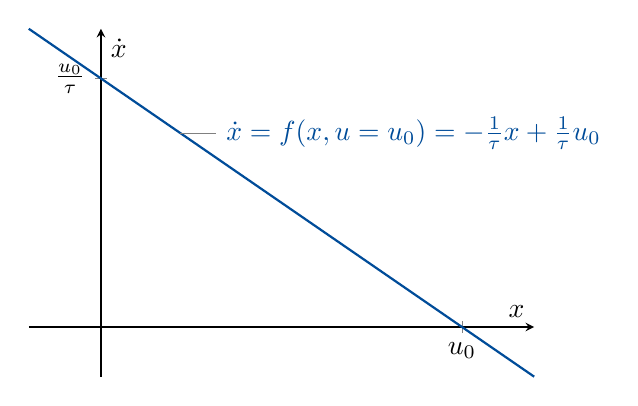
\begin{tikzpicture}
    \pgfmathsetmacro{\tconst}{2}
    \pgfmathsetmacro{\kgain}{1}
    \pgfmathsetmacro{\uconst}{1}
    \pgfmathsetmacro{\xmax}{\uconst}
    \pgfmathsetmacro{\ymax}{\uconst/\tconst}
    \begin{axis}[
      %yshift=-5cm,
      clip=false,
      axis lines=middle,
      width = 8cm,
      height = 6cm,
      xlabel = {$x$},
      ylabel = {$\dot{x}$},
      xtick={0, \xmax},
      xticklabels={0, $u_0$},
      ytick={0, \ymax},
      yticklabels={0, $\frac{u_0}{\tau}$},
      %title={$\dot{x} = f(x) = -\frac{1}{\tau} x + \frac{1}{\tau}u_0$},
      ]
      \addplot[outputclr, thick, no marks, domain=-0.2:\xmax+0.2, samples=10] {-1.0/\tconst * x + 1.0/\tconst * \uconst} node[coordinate, pin=0:{$\dot{x}=f(x,u=u_0) = -\frac{1}{\tau} x + \frac{1}{\tau}u_0$}, pos=0.3] {};
    \end{axis}
  \end{tikzpicture}
\end{center}
\end{column}
\end{columns}
\end{frame}

\begin{frame}[label={sec:org3599a14}]{Another relevant first-order system: Logistic growth}
\[ \dot{x} = \underbrace{a\big(1 - \frac{x}{x_{max}}\big)x}_{f(x)} \]

\begin{center}
  \begin{tikzpicture}
    \pgfmathsetmacro{\gconst}{2}
    \pgfmathsetmacro{\xmax}{1}
    \pgfmathsetmacro{\ymax}{\gconst*\xmax/4}
    \begin{axis}[
      %yshift=-5cm,
      clip=false,
      axis lines=middle,
      width = 8cm,
      height = 6cm,
      xlabel = {$x$},
      ylabel = {$\dot{x}$},
      xtick={0, \xmax},
      xticklabels={0, $x_{max}$},
      ytick={0, \ymax},
      yticklabels={0, $a\frac{x_{max}}{4}$},
      ymax=\ymax+0.1,
      xmax=\xmax+0.1,
      %title={$\dot{x} = f(x) = -\frac{1}{\tau} x + \frac{1}{\tau}u_0$},
      ]
      \addplot[outputclr, thick, no marks, domain=-0.05:\xmax+0.05, samples=100] {\gconst * (1- x/\xmax)*x} node[coordinate, pin=0:{$\dot{x}=f(x) = a\big(1 - \frac{x}{x_{max}}\big)x$}, pos=0.7] {};
    \end{axis}
  \end{tikzpicture}
\end{center}
{\footnotesize See 3Blue1Brown \texit{Exponential growth and epidemics} \url{https://youtu.be/Kas0tIxDvrg}}
\end{frame}

\begin{frame}[label={sec:orgf8836be}]{Do in groups}
\begin{center}
  \begin{tikzpicture}
    \pgfmathsetmacro{\gconst}{2}
    \pgfmathsetmacro{\xmax}{1}
    \pgfmathsetmacro{\ymax}{\gconst*\xmax/4}
    \begin{axis}[
      %yshift=-5cm,
      clip=false,
      axis lines=middle,
      width = 8cm,
      height = 6cm,
      xlabel = {$x$},
      ylabel = {$\dot{x}$},
      xtick={0, \xmax},
      xticklabels={0, $x_{max}$},
      ytick={0, \ymax},
      yticklabels={0, $a\frac{x_{max}}{4}$},
      ymax=\ymax+0.1,
      xmax=\xmax+0.1,
      %title={$\dot{x} = f(x) = -\frac{1}{\tau} x + \frac{1}{\tau}u_0$},
      ]
      \addplot[outputclr, thick, no marks, domain=-0.05:\xmax+0.05, samples=100] {\gconst * (1- x/\xmax)*x} node[coordinate, pin=0:{$\dot{x}=f(x) = a\big(1 - \frac{x}{x_{max}}\big)x$}, pos=0.7] {};
    \end{axis}
  \end{tikzpicture}
\end{center}
\begin{enumerate}
\item In breakout rooms: One of you shares this slide (found on canvas, link in the program for the session)
\item Sketch the solution \(x(t)\) using the "bead-on-a-wire" idea for the inital value problem \(x(0) = 0.1x_{max}\).
\end{enumerate}
\end{frame}

\section{Linearization}
\label{sec:org14863e2}
\begin{frame}[label={sec:org43156cb}]{The general idea}
Given a dynamical system described by a nonlinear differential equation
\begin{center}
  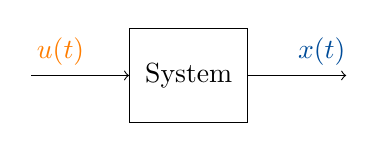
\begin{tikzpicture}[node distance=22mm, block/.style={rectangle, draw, minimum width=15mm, minimum height=12mm}, sumnode/.style={circle, draw, inner sep=2pt}]

    \node[coordinate] (input) {};
    \node[block, right of=input, node distance=20mm] (plant)  {System};
    \node[coordinate, right of=plant, node distance=20mm] (output) {};

    \draw[->] (input) -- node[above, pos=0.3, color=inputclr] {$u(t)$} (plant);
    \draw[->] (plant) -- node[above, near end, color=outputclr] {$x(t)$} (output);
  \end{tikzpicture}
\end{center}   
\[ \dot{\textcolor{outputclr}{x}} = f(\textcolor{outputclr}{x}, \textcolor{inputclr}{u})\]

Find a linear approximation to the differential equation about an \alert{operating point} \((\textcolor{outputclr}{x_0}, \, \textcolor{inputclr}{u_0})\)
\end{frame}

\begin{frame}[label={sec:org5f5417f}]{The general picture}
\begin{center}
  \begin{tikzpicture}
    \pgfmathsetmacro{\xnoll}{1.5}
    \pgfmathsetmacro{\xmax}{2}
    \pgfmathsetmacro{\fnoll}{sqrt(2-\xnoll)}
    \begin{axis}[
      %yshift=-5cm,
      clip=false,
      axis lines = middle,
      width = 12cm,
      height = 8cm,
      %xlabel = {$x$},
      %ylabel = {$\dot{x}$},
      xtick={0, \xnoll, \xmax},
      xticklabels={0, $x_0$, $x_{max}$},
      ytick={0},
      %title={$\dot{x} = f(x) = \sqrt{x_{max} -  x}$},
      ]
      \addplot[outputclr, thick, no marks, domain=0:\xmax, samples=100] {sqrt(\xmax-x)} node[coordinate, pin=-120:{$\dot{x}=f(x)= \sqrt{x_{max} -  x}$}, pos=0.1] {};
      \addplot[green!70!black, thick, no marks, domain=0.8:\xmax, samples=10] {sqrt(\xmax-\xnoll) - 0.5/sqrt(\xmax-\xnoll)*(x-\xnoll)} node[coordinate, pin=0:{$\dot{x}\approx f(x_0) + \frac{d}{dx}f|_{x_0}(x-x_0)$}, pos=0.1] {};
      \node[coordinate, pin=180:{$f(x_0)$},] at (axis cs: 0.02, \fnoll) {};
      \node at (axis cs: -0.3, 1.5) {$\dot{x}$};
      \node at (axis cs: 1.9, -0.3) {$x$};
      %\node[coordinate, pin=-90:{$x_0$},] at (axis cs: \xnoll, -0.2) {};
    \end{axis}

  \end{tikzpicture}
\end{center}
\end{frame}

\begin{frame}[label={sec:orgcb3dd14}]{Linearizing the tank-valve nonlinear model}
\[ \dot{p} = a_0(u_v - 5)|p_s - p|^{a_1} = f(p, u_v), \quad \text{with} \; a_0=1.1\; \text{and}\; a_1 = 0.47\]
\begin{enumerate}
\item Given operating pressure \(p_0\). Choose operating point \(u_0\) which gives equilibrium \(f(p_0, u_0) = 0\).
\end{enumerate}
\end{frame}


\begin{frame}[label={sec:org56a6724}]{Linearizing the tank-valve nonlinear model}
\[ \dot{p} = a_0(u_v - 5)|p_s - p|^{a_1} = f(p, u_v), \quad \text{with} \; a_0=1.1\; \text{and}\; a_1 = 0.47\]
\begin{enumerate}
\item Given operating pressure \(p_0\). Choose operating point \(u_0\) which gives equilibrium \(f(p_0, u_0) = 0\).
\item Introduce deviation variables: \(u_v = 5 + \textcolor{inputclr}{u}\) and \(p = p_0 + \textcolor{outputclr}{y}\).
\end{enumerate}
\end{frame}


\begin{frame}[label={sec:orga9fd2fc}]{Linearizing the tank-valve nonlinear model}
\[ \dot{p} = a_0(u_v - 5)|p_s - p|^{a_1} = f(p, u_v), \quad \text{with} \; a_0=1.1\; \text{and}\; a_1 = 0.47\]
\begin{enumerate}
\setcounter{enumi}{2}
\item Determine partial derivatives
\begin{align*}
\frac{\partial f}{\partial p} &= a_0(u_v-5)a_1|p_s - p|^{a_1-1}(-1)\\
\frac{\partial f}{\partial u_v} &= a_0|p_s - p|^{a_1}
\end{align*}
\item Evaluate partial derivatives at the operating point \((p_0, u_0\).
\begin{align*}
\frac{\partial f}{\partial p}\big|_{p_0, u_0} &= 0\\
\frac{\partial f}{\partial u_v}\big|_{p_0, u_0} &=  a_0|p_s - p_0|^{a_1}
\end{align*}
\end{enumerate}
\end{frame}




\begin{frame}[label={sec:orgadabd43}]{Linearizing the tank-valve nonlinear model}
\[ \dot{p} = a_0(u_v - 5)|p_s - p|^{a_1} = f(p, u_v), \quad \text{with} \; a_0=1.1\; \text{and}\; a_1 = 0.47\]
\begin{enumerate}
\setcounter{enumi}{3}
\item Evaluate partial derivatives at the operating point \((p_0, u_0\).
\begin{align*}
\frac{\partial f}{\partial p}\big|_{p_0, u_0} &= 0\\
\frac{\partial f}{\partial u_v}\big|_{p_0, u_0} &=  a_0|p_s - p_0|^{a_1}
\end{align*}
\item Form the linearized model
\begin{equation}
\begin{aligned} \dot{p} = \dot{\textcolor{outputclr}{y}} &= f(p, u_v) \approx f(p_0, u_0) + \frac{\partial f}{\partial p}|_{p_0, u_0}(p-p_0) + \frac{\partial f}{\partial u_v}|_{p_0, u_0}(u_v - u_0)\\
 &=  a_0|p_s - p_0|^{a_1} \textcolor{inputclr}{u}.
\end{aligned}
\end{equation}
\end{enumerate}
\end{frame}

\begin{frame}[label={sec:orgccfd0c1}]{Linearizing the tank-valve nonlinear model}
We arrive at the linear model
\begin{equation*}
\begin{aligned}
 \dot{\textcolor{outputclr}{y}} &= a_0|p_s - p_0|^{a_1} \textcolor{inputclr}{u}, \qquad \text{which in the Laplace domain is}\\[4mm]
 \textcolor{outputclr}{Y(s)} &= \frac{a_0|p_s - p_0|^{a_1}}{s} \textcolor{inputclr}{U(s)}    
\end{aligned}
\end{equation}
\end{frame}



\begin{frame}[label={sec:orgdf6bf5d}]{Do in groups}
\[ \dot{p} = a_0(u_v - 5)|p_s - p|^{a_1}\; \textcolor{red!90!black}{-\, v} = f(p, u_v)\]

\begin{enumerate}
\item Given operating pressure \(p_0\). Choose operating point \(u_0\) which gives equilibrium \(f(p_0, u_0) = 0\).
\item Introduce deviation variables: \(u_v = u_0 + \textcolor{inputclr}{u}\) and \(p = p_0 + \textcolor{outputclr}{y}\).
\item Determine partial derivatives.
\item Evaluate partial derivatives at the operating point.
\item Form the linearized model
\end{enumerate}
\end{frame}
\end{document}